\documentclass[11pt]{article}
\usepackage[T1]{fontenc}
\usepackage{amsmath,amssymb,amsthm,mathtools}
\usepackage{booktabs,tabularx}
\usepackage{tikz}
\usetikzlibrary{arrows.meta,positioning}
\usepackage[a4paper,margin=1in]{geometry}
\usepackage[hidelinks]{hyperref}
\usepackage[expansion=false]{microtype}
\emergencystretch=2em

\newtheorem{definition}{Definition}[section]
\newtheorem{lemma}[definition]{Lemma}
\newtheorem{proposition}[definition]{Proposition}
\newtheorem{theorem}[definition]{Theorem}
\newtheorem{corollary}[definition]{Corollary}
\newtheorem{conjecture}[definition]{Conjecture}
\theoremstyle{remark}
\newtheorem{remark}[definition]{Remark}

\title{Experiments with Theta Cycles Modulo $p^2$:\\
Hasse-Jet Duality and a Shifted-Conic Conjecture}
\author{Jeffery Opoku\\
\small School of Mathematical and Statistical Sciences\\
\small University of Texas Rio Grande Valley, Edinburg, Texas 78539, USA\\
\small \texttt{jeffery.opoku01@utrgv.edu}}
\date{4 October 2026}

\begin{document}
\maketitle

\begin{abstract}
We study the unresolved weight filtration of theta iterates modulo $p^2$
with exact computation.  In $692$ ordinary cross-wedge cells, one shifted
quadratic matches every interior obstruction.  All $234$ failures lie on
three affine boundary lines.  Two further tests give $2{,}324$ exact matches
with one factorial boundary scalar.  We also prove four facts.  The
obstruction is a first Hasse jet.  The relevant Hasse quotients have a
perfect pairing.  Theta is skew-adjoint for this pairing.  The
minimal-weight projection is explicit, and exact filtration separates the
boundary directions.  These facts reduce the shifted-conic law to one
factorial block identity and two endpoint identities.  We state these open
identities as conjectures.  The paper includes code, negative controls, and
exact tests that could disprove them.
\end{abstract}

\noindent\textbf{Keywords:} theta cycles; modular forms modulo prime powers;
experimental mathematics; Hasse invariant; Bockstein class; weight
filtration.

\noindent\textbf{2020 Mathematics Subject Classification:}
11F33, 11F11, 11Y40.

\section{Introduction}

The theta cycle of a modular form modulo a prime is classical.  Modulo
$p^2$, weight lowering contains a new first-order obstruction: a form that
lowers in weight modulo $p$ need not admit the same lowering modulo $p^2$.
Ahlgren, Raum, and Richter determined the initial segment and many later
parts of the cycle \cite{ARR2026}.  Some low points in the next band are
still not known for all primes.

We began with one exact question.  Does the quadratic pattern in the
resolved wedge remain valid after reflection into the next wedge?  The
first candidate failed on every tested $D=0$ cell.  We then added the
missing minimal-weight projection.  In the interior, the lower Bockstein
class was controlled by
\begin{equation}\label{eq:intro-shifted-conic-experimental}
 i'^2+(k-1)i'-(n+1)(n+2)\quad\text{in }\mathbb F_p.
\end{equation}
All disagreements occurred on three affine lines.  Their full residuals
then suggested one factorial block and two triangular endpoint formulas.

The paper records how this formula was found and how it was tested.  The
calculation uses exact modular arithmetic and Sturm-safe remainders.  It
also includes a failed baseline, a blind prime extension, and a separate
test in a two-dimensional cusp-form space.  We then prove the geometric
facts behind the experiment.  The weight-lowering obstruction is a first
Hasse jet.  The ambient quotient has a perfect pairing, and theta is
skew-adjoint.  Multiplication by the integral Hasse inclusion commutes with
theta modulo $p^2$.  We also give an explicit formula for the minimal-weight
projection.  Exact filtration separates the proposed boundary directions.

The open part is small but important.  The first-Hasse-jet formula should
reduce to a factorial block identity.  This identity would imply the generic
shifted-conic law and the observed scalar on the third line.  Two endpoint
coefficients remain open on the other boundary lines.  We do not call these
statements theorems because the present evidence is finite.

The experiments are part of the main argument.  They identify the
classification problem and the three boundary cases.  The theorems explain
the form of the candidate and reduce the open part to explicit identities.

\subsection{Relation to prior work}

Ahlgren--Raum--Richter \cite{ARR2026} prove the initial segment, further
exact values or bounds modulo $p^2$, and a quadratic condition for the
exceptional positions in their resolved region.  For comparison, the
included code checks the resolved $D=2$ subwedge, whose conic is
\[
 i'^2+(k-1)i'-n(n+1)=0.
\]
The present experiment studies the complementary $D=0$ subwedge.
Reflection changes the constant term to $(n+1)(n+2)$.  A new first-Hasse-jet
projection is needed before this expression gives the actual obstruction.
The result is not a restatement of Ahlgren--Raum--Richter, and the geometric
pairing alone does not prove the shifted-conic law.

\subsection{Guide to the paper}

Section~\ref{sec:experimental-design} states the finite experiment, its
negative controls, validation layers, and failure criteria.  The next two
sections develop the first-Hasse-jet and direct block calculations.
Section~\ref{sec:experimental-interpretation} separates what the experiments
establish from what remains open.  The final sections formulate the
shifted-conic consequences, summarize theorem status, and give commands for
exact reproduction.

\section{Experimental design and discovery path}
\label{sec:experimental-design}

\subsection{Objects, arithmetic, and inclusion rules}

The experiment concerns the filtration of $\theta^i f$ modulo $p^2$ for
ordinary level-one modular forms of weight $4\leq k<p-1$.  Every reported
comparison uses exact integer arithmetic.  Fourier expansions are retained
past the Sturm bound at each relevant weight, so equality of the retained
series is an exact equality of modular forms in the tested case.  No
floating-point approximation, numerical tolerance, random sampling, or
model fitting is used.

The computational record contains $5{,}572$ cells.  Of these, $5{,}434$
satisfy the ordinary condition $k<p-1$.  The main experiment
uses the $692$ ordinary, nondegenerate cells for which a $D=0$ index and its
Tate complement lie in the proved $D=2$ wedge.  These cells range over
primes $17\leq p\leq43$ and weights $8\leq k\leq22$.  A cell is included by
these arithmetic conditions alone, before its obstruction class or the
value of the candidate quadratic is inspected.

For each cell, the program performs four exact operations:
\begin{enumerate}
\item reduce $\theta^if$ modulo $p^2$ against an integral echelon basis of
      $M_{w_-}$;
\item divide the resulting canonical remainder by $p$ and reduce modulo
      $p$, producing the lower Bockstein class $\mathcal B_i$;
\item independently construct the shifted leading-block candidate
      \[
      \mathcal L_i=q_1(n,i')X^p\theta^{i-p}f,
      \qquad
      q_1(n,i')=i'^2+(k-1)i'-(n+1)(n+2);
      \]
\item compare the complete canonical remainders, not a selected coordinate
      or a short Fourier prefix.
\end{enumerate}
The program records both agreements and failures.  For each failure, it
stores the full residual
$\mathcal B_i-\mathcal L_i$ whenever the proposed identity fails.

\subsection{How the pattern was found}

We found the pattern in stages.  The first candidate reused the $D=2$
formula one Hasse step lower.  It failed in all $1{,}593$ ordinary,
nondegenerate $D=0$ cells.  This negative control showed that a new
first-order correction was needed.

Reflection to the complementary wedge then suggested replacing the earlier
quadratic $i'^2+(k-1)i'-n(n+1)$ by $q_1(n,i')$.  On the $692$ cross-wedge
cells, the resulting class agreed with the direct Bockstein in $458$ cases.
The $234$ disagreements did not scatter: they were exactly the cells on
the three affine lines
\[
 i'=n+2,
 \qquad i'+n=2p-k-1,
 \qquad i'+n=2p-k.
\]
Each line contains $78$ cells.  Away from these lines, the direct class
vanished in exactly $20$ cases, and these were exactly the cases
$q_1(n,i')=0$.  Thus the shifted conic was found only after the first
formula failed and the full residuals identified the three boundary cases.

The boundary residuals suggested further exact formulas.  On $i'=n+2$ the
residual always occupied one explicit block direction, and rational
reconstruction across primes produced the scalar
\[
 -m(k-2m-2)!,\qquad m=p-2-n.
\]
On the two triangular lines, exact elimination placed every residual in an
explicit triangular span and recovered endpoint coefficient $-(m+1)$.
These results led to the Hasse-jet and filtration arguments proved below.

\begin{figure}[t]
\centering
\resizebox{0.98\linewidth}{!}{%
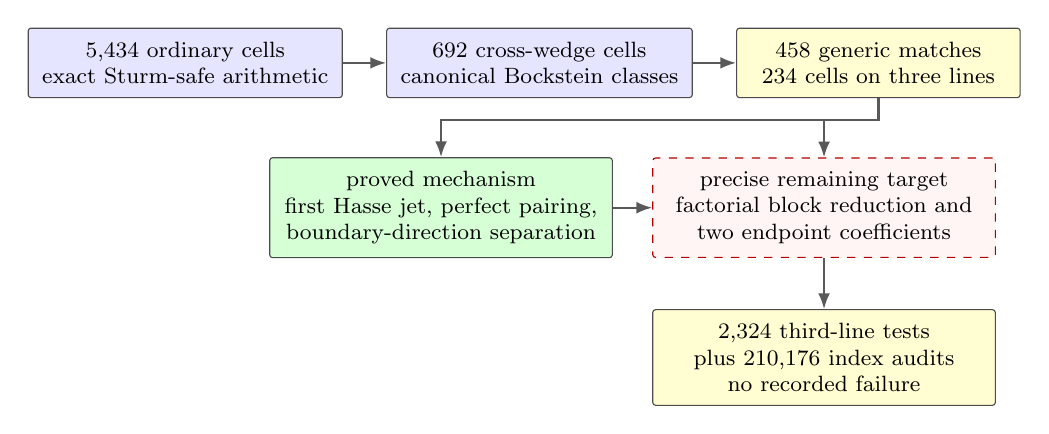
\begin{tikzpicture}[
  font=\footnotesize,
  box/.style={draw=black!70, rounded corners=1pt, align=center,
              minimum height=0.85cm, inner sep=5pt},
  data/.style={box, fill=blue!10},
  found/.style={box, fill=yellow!18},
  proved/.style={box, fill=green!16},
  open/.style={box, draw=red!70!black, dashed, fill=red!4},
  flow/.style={-{Latex[length=2mm]}, thick, draw=black!65}
]
\node[data, minimum width=3.3cm] (record) at (0,0)
  {$5{,}434$ ordinary cells\\exact Sturm-safe arithmetic};
\node[data, minimum width=3.3cm, right=0.55cm of record] (wedge)
  {$692$ cross-wedge cells\\canonical Bockstein classes};
\node[found, minimum width=3.6cm, right=0.55cm of wedge] (pattern)
  {$458$ generic matches\\$234$ cells on three lines};
\draw[flow] (record) -- (wedge);
\draw[flow] (wedge) -- (pattern);

\node[proved, minimum width=4.35cm, below=0.75cm of wedge, xshift=-1.25cm]
  (theory) {proved mechanism\\first Hasse jet, perfect pairing,\\boundary-direction separation};
\node[open, minimum width=4.35cm, right=0.5cm of theory]
  (conjecture) {precise remaining target\\factorial block reduction and\\two endpoint coefficients};
\draw[flow] (pattern.south) -- ++(0,-0.28) -| (theory.north);
\draw[flow] (pattern.south) -- ++(0,-0.28) -| (conjecture.north);
\draw[flow] (theory) -- (conjecture);

\node[found, minimum width=4.35cm, below=0.65cm of conjecture]
  (tests) {$2{,}324$ third-line tests\\plus $210{,}176$ index audits\\no recorded failure};
\draw[flow] (conjecture) -- (tests);
\end{tikzpicture}
}
\caption{The experiment-to-theorem path.  Exact computation first isolated
the generic quadratic and its three boundary lines.  The green box records
the uniform results proved here.  The dashed box is the remaining symbolic
identity; finite tests support it but do not prove it.}
\label{fig:experimental-workflow}
\end{figure}



\subsection{Validation and negative controls}

Table~\ref{tab:experimental-audit} separates discovery calculations,
blind extensions, independent form tests, and symbolic-index audits.  A
zero failure count means that the stated exact identity held throughout the
specified finite range.  It does not convert the identity into a theorem
for arbitrary primes.

\begin{table}[t]
\centering
\small
\renewcommand{\arraystretch}{1.13}
\begin{tabularx}{\linewidth}{@{}>{\raggedright\arraybackslash}p{0.25\linewidth}>{\raggedright\arraybackslash}p{0.22\linewidth}>{\raggedright\arraybackslash}X@{}}
\toprule
Audit & Exact range & Outcome\\
\midrule
Ordinary-cell census & $5{,}434$ cells & Establishes the ambient finite
record and its admissible subfamilies.\\
Naive lower-block control & $1{,}593$ $D=0$ cells & The reused $D=2$
formula failed in all cells, isolating the missing projection term.\\
Cross-wedge discovery & $692$ cells & $458$ interior matches, $234$
boundary disagreements, and $20$ shifted-conic zeros.\\
Explicit first-Hasse-jet lift & The same $692$ cells & No weight,
mod-$p$, or canonical-Bockstein mismatch.\\
Third-line blind extension & $652$ cells through $p=79$ & No zero
residual, block-shape failure, or factorial-scalar mismatch.\\
Independent weight-$24$ forms & $186$ ordinary forms and $1{,}860$ tests
through $p=43$ & No zero residual, block-shape failure, or scalar mismatch.\\
Triangular endpoints & $156$ boundary cells & Endpoint rank increased by
one and the coefficient was $-(m+1)$ in every case.\\
Index and filtration audit & $210{,}176$ parameter cells through $p=101$ &
No exponent, weight, pairing, or filtration-gap failure.\\
Affine-reduction audit & $614$ factorial-range cells and $156$ recurrence
steps & No coefficient, sign, or low-point branch failure.\\
\bottomrule
\end{tabularx}
\caption{Exact audits used in the discovery and validation of the proposed
shifted-conic mechanism.  The two large validation experiments were written
as falsification tests: they count zero residuals, shape failures, and scalar
mismatches separately.}
\label{tab:experimental-audit}
\end{table}

The weight-$24$ experiment is important because the relevant cusp-form
space is two-dimensional.  It tests two generators and their projective
linear combinations rather than repeating the calculation on a single
one-dimensional family.  The third-line extension is also separate from
the original $78$ boundary cells: it searches new primes and weights after
the one-block shape and factorial scalar have been specified.

\subsection{What would falsify the conjectural mechanism}

Each computational claim has a direct failure test.  Any of the following
would disprove part of the proposed mechanism:
\begin{enumerate}
\item an interior cross-wedge cell with
      $\mathcal B_i\neq q_1(n,i')X^p\theta^{i-p}f$;
\item a cell with $q_1(n,i')=0$ and nonzero interior Bockstein, or an
      interior zero with $q_1(n,i')\neq0$;
\item a third-line residual outside the predicted one-block direction;
\item a third-line scalar different from $-m(k-2m-2)!$ or dependent on the
      chosen ordinary form;
\item a triangular residual outside the stated span or with endpoint
      coefficient different from $-(m+1)$.
\end{enumerate}
The released scripts report each failure type separately.  The tests remain
useful even though the factorial block reduction is still open.


\section{Notation and proof roadmap}\label{sec:notation-roadmap}

\subsection{Core notation}

The symbols used repeatedly in the proof are collected here.  The band
level $D(i)$ is included explicitly so that the later references to the
$D=0$ and $D=2$ strata are self-contained.

\begingroup
\renewcommand{\arraystretch}{1.16}
\noindent\begin{tabularx}{\linewidth}{@{}>{$}l<{$}>{\raggedright\arraybackslash}X@{}}
\toprule
\text{Symbol} & \text{Meaning}\\
\midrule
p,\ k,\ f & $p\geq5$ is prime; $f$ is an ordinary level-one form of weight
$4\leq k<p-1$.\\
\theta,\ \omega_{p^a} & The operator $q\,d/dq$ and weight filtration modulo
$p^a$, respectively.\\
i=np+i' & Band index, with $n$ the segment number and $i'$ the position
inside the segment.\\
P & The full Hasse drop $p(p-1)$.\\
D(i) & The least integer $D$ such that
$k+2i+DP\geq\omega_p(\theta^{i-p}f)+p(p+1)$; this is the inherited band
upper-bound level.\\
w_- & The candidate lower weight $k+2i-P$ in the $D=0$ stratum.\\
A,\ S,\ Z & $A=E_{p-1}$ is the chosen integral lift of the Hasse invariant,
$S=\operatorname{div}(A\bmod p)$, and $Z=pS$ is its length-$p$ thickening.\\
Q_r & The Hasse quotient
$H^0(Z,\omega^r|_Z)\simeq
M_r(\mathbb F_p)/A^pM_{r-P}(\mathbb F_p)$.\\
\mathcal B_i,\ \mathcal L_i & The Bockstein class of $\theta^if$ at weight
$w_-$ and its shifted leading-block candidate.  Their difference is the
boundary residual.\\
X & The divided Eisenstein series $E_2/12$ modulo $p$; powers of $X$ form
the direct block basis used in the reduction.\\
\alpha,\ \Phi_r,\ \eta_r & The first Hasse jet $(A-1)/p$, the periodicity
quotient $(\theta^{r+p-1}f-\theta^rf)/p$, and the lift error
$(G_r-\theta^rf)/p$, all reduced modulo $p$.\\
Z_d & The block direction $X^d\theta^{p-k}f$ in the factorial reduction.\\
i^\dagger & The complementary index $p^2+1-k-i$ used in the Tate-dual
comparison.\\
\bottomrule
\end{tabularx}
\endgroup

\paragraph{Terminology.}
A \emph{first Hasse jet} is a class on the thickened Hasse divisor $Z$.
A \emph{Bockstein class} is the intrinsic obstruction to an integral
weight-lowering lift.  A \emph{minimal-weight projection} is a chosen
characteristic-zero representative of the smallest candidate weight.  The
\emph{block basis} is the direct basis built from powers of $X$ and theta
iterates.  A \emph{boundary residual} is the difference between the
Bockstein class and its shifted leading-block candidate on one of the three
affine boundary lines.

\subsection{Dependency roadmap}

The proof has five logically separate layers.  The first three are uniform
in the admissible parameters and do not use the conjectural scalar identity.

\begingroup
\renewcommand{\arraystretch}{1.16}
\small
\noindent\begin{tabularx}{\linewidth}{@{}>{\raggedright\arraybackslash}p{0.15\linewidth}>{\raggedright\arraybackslash}p{0.31\linewidth}>{\raggedright\arraybackslash}X@{}}
\toprule
Layer & Main result & Logical role\\
\midrule
Geometric & Perfect Hasse-quotient duality and theta skew-adjointness &
Uses duality on $Z$; independent of all finite computations and block
formulas.\\
Integral & Bockstein realization, Hasse inclusion, and the explicit
periodic first-Hasse-jet formula & Uses integral Eisenstein lifts and the
first ordinary low-point congruence; supplies the minimal-weight projection.\\
Filtration & Uniform separation of all three boundary directions and
nonvanishing of the factorial scalar candidate & Uses exact mod-$p$
filtration; independent of the factorial block reduction.\\
Computational & Exact classification of $692$ cross-wedge cells and
$2{,}324$ third-line stress tests & Proved only on the deposited finite
range; discovers and falsifies formulas but is not extrapolated to all $p$.\\
Conditional & Factorial block reduction and two triangular endpoint
coefficients & Would identify the actual boundary residuals and imply the
shifted-conic filtration law.\\
\bottomrule
\end{tabularx}
\endgroup

Thus the dependency chain is
\[
\begin{aligned}
 \boxed{\text{geometry}}+\boxed{\text{integral first Hasse jet}}
 &\Longrightarrow \boxed{\text{explicit Bockstein class}},\\
 \boxed{\text{explicit Bockstein class}}
 &\xRightarrow[\text{open}]{\text{block reduction}}
 \boxed{\text{shifted-conic law}}.
\end{aligned}
\]
The boundary-separation theorem branches from the filtration layer before
the open implication and therefore remains unconditional.


\section{Bocksteins and Hasse quotients}
\subsection{The weight-lowering Bockstein}

Let $R=\mathbb Z_{(p)}$, and let $M_w(R)$ denote the space of level-one
modular forms of weight $w$ with coefficients in $R$.  We identify a form
with its $q$-expansion.  Write
\[
  \overline M_w:=M_w(R)/pM_w(R)
\]
and let $\overline{\mathcal D}$ be the space of divided congruences modulo
$p$, viewed through their $q$-expansions.

\begin{definition}\label{def:bockstein}
Let $g\in\mathcal D(R/p^2R)$ and suppose that $g\pmod p$ is represented by
some $h\in M_w(R)$.  Define
\[
  \beta_w(g):=\left[\frac{g-h}{p}\right]
       \in \overline{\mathcal D}/\overline M_w.
\]
Here any lift of the $q$-expansion of $g$ to $R$ may be used in the
numerator.
\end{definition}

\begin{lemma}\label{lem:bockstein}
The class $\beta_w(g)$ is independent of the choices in Definition
\ref{def:bockstein}.  Moreover,
\[
  \beta_w(g)=0
  \quad\Longleftrightarrow\quad
  g\equiv H\pmod{p^2}
  \quad\text{for some }H\in M_w(R).
\]
Consequently, if $w$ lies in the admissible weight class of $g$, then
\[
  \beta_w(g)=0
  \quad\Longleftrightarrow\quad
  \omega_{p^2}(g)\le w.
\]
\end{lemma}

\begin{proof}
Suppose first that $h,h'\in M_w(R)$ both represent $g\pmod p$.  Then
$h-h'$ has $q$-expansion divisible by $p$.  The $q$-expansion lattice
$M_w(R)$ is saturated: an integral modular form whose coefficients are all
divisible by $p$ belongs to $pM_w(R)$.  One can also see this directly by
forward substitution in the standard integral echelon basis, whose pivot
coefficients are units.  Thus $h-h'\in pM_w(R)$.  Hence
\[
  \frac{g-h}{p}-\frac{g-h'}{p}=\frac{h'-h}{p}\in M_w(R),
\]
so the two choices define the same class modulo $\overline M_w$.  Changing
the integral lift of $g$ changes the quotient by an arbitrary multiple of
$p^2/p=p$, and hence does not change its reduction modulo $p$.  This proves
well-definedness.

If $\beta_w(g)=0$, there is an $m\in M_w(R)$ such that
$(g-h)/p\equiv m\pmod p$.  Thus
\[
  g\equiv h+pm\pmod{p^2},
\]
and $h+pm$ belongs to $M_w(R)$.  Conversely, suppose that
$g\equiv H\pmod{p^2}$ for some $H\in M_w(R)$.  Since
$H\equiv h\pmod p$, the same echelon-basis argument gives
$H-h=pm$ for some $m\in M_w(R)$.  It follows that
\[
  \frac{g-h}{p}\equiv\frac{H-h}{p}=m\pmod p,
\]
so $\beta_w(g)=0$ in
$\overline{\mathcal D}/\overline M_w$.  For the final equivalence, assume
that every smaller admissible representative weight differs from $w$ by a
nonnegative multiple of $P=p(p-1)$.  Multiplication by the corresponding
power of $E_{p-1}^p\equiv1\pmod {p^2}$ raises such a representative to
weight $w$ without changing its reduction modulo $p^2$.  Therefore a
representative of weight at most $w$ exists exactly when one of weight $w$
exists.  This is the asserted filtration criterion.
\end{proof}

\begin{remark}\label{rem:bockstein-computation}
The canonical echelon remainder used in the computations is a coordinate
representative of $\beta_w(g)$.  Reducing $g$ modulo the integral echelon
basis of $M_w(R)$ kills the same leading coefficients as the lift $h$ in
the proof.  The resulting remainder is divisible by $p$, and division by
$p$ followed by reduction modulo $p$ gives the displayed class.  Thus the
computational zero test is intrinsic even though its coordinate vector
depends on the chosen echelon basis.
\end{remark}

\subsection{Hasse duality and the Eisenstein bridge}

Let $p\geq5$, put $P=p(p-1)$, and work first on a compactified Katz
modular curve $X$ with auxiliary full level $3$. Let $\omega$
be the Hodge bundle, let $C$ be the cusp divisor, and let
$A\in H^0(X,\omega^{p-1})$ be the Hasse invariant. Its zero divisor
$S$ is reduced and disjoint from $C$. Put $Z=pS$, so that $Z$ is the
Cartier divisor cut out by $A^p$. For every integer $r$ define
\[
 \mathcal Q_r:=\omega^r/A^p\omega^{r-P}
              \simeq \omega^r\vert_Z,
 \qquad Q_r:=H^0(Z,\mathcal Q_r).
\]
The constructions below commute with the tame deck group. Its order is
prime to $p$, so the Reynolds operator is exact.  The canonical pairing
below is deck-invariant, and its restriction to invariant subspaces is
perfect.  This gives the same statement at level one.  Equivalently, one
may formulate it directly on the tame compactified moduli stack.

\begin{proposition}[Perfect Hasse-quotient pairing]
\label{prop:hasse-perfect-pairing}
For every $r$ there is a canonical perfect pairing
\[
 \langle\ ,\ \rangle_r:
 Q_r\times Q_{P+2-r}\longrightarrow \mathbb F_p.
\]
It is the product pairing followed by the trace map on the finite
Gorenstein scheme $Z$.
\end{proposition}

\begin{proof}
Because $Z$ is an effective Cartier divisor on the smooth curve $X$, its
dualizing sheaf is
\[
 \omega_Z\simeq\bigl(\omega_X\otimes\mathcal O_X(Z)\bigr)\vert_Z.
\]
Kodaira--Spencer gives $\omega_X(C)\simeq\omega^2$, while
$\mathcal O_X(Z)\simeq\omega^P$. The canonical section of
$\mathcal O_X(C)$ is nonzero on $Z$, since $C\cap Z=\varnothing$.
Consequently
\[
 \omega_Z\simeq\omega^{P+2}\vert_Z.
\]
Multiplication now gives
\[
 \mathcal Q_r\otimes\mathcal Q_{P+2-r}\longrightarrow\omega_Z.
\]
Composing global sections with
$\operatorname{Tr}_Z:H^0(Z,\omega_Z)\to\mathbb F_p$ gives the displayed
pairing. Duality for the finite Gorenstein scheme $Z$ identifies
$\mathcal Q_{P+2-r}$ with
$\mathcal Hom_Z(\mathcal Q_r,\omega_Z)$, so the pairing is perfect.
\end{proof}

Let $\Theta$ denote the Katz theta operator in characteristic $p$,
normalized by its $q$-expansion
\[
 \Theta\!\left(\sum a_nq^n\right)=\sum n a_nq^n.
\]
It raises weight by $p+1$, satisfies the product rule, and satisfies
$\Theta(A)=0$. Hence it induces
\[
 \Theta:Q_r\longrightarrow Q_{r+p+1}.
\]

\begin{proposition}[Theta adjointness]
\label{prop:theta-adjointness}
If $x\in Q_r$ and $y\in Q_{P+1-p-r}$, then
\[
 \langle\Theta x,y\rangle_{r+p+1}
   =-\langle x,\Theta y\rangle_r.
\]
More generally, for $m\geq0$ and
$y\in Q_{P+2-r-m(p+1)}$,
\[
 \langle\Theta^m x,y\rangle_{r+m(p+1)}
   =(-1)^m\langle x,\Theta^m y\rangle_r.
\]
\end{proposition}

\begin{proof}
The two products in the first formula have weight $P+2$, so both traces
are defined. The product rule gives
\[
 (\Theta x)y+x(\Theta y)=\Theta(xy).
\]
Notice that $xy$ has weight
\[
 P+1-p=(p-1)^2.
\]
Let $a$ be the canonical section on the Igusa curve, normalized by
$a^{p-1}=A$. The differential attached to $\Theta(xy)$ is
$\Theta(xy)/a^P=\Theta(xy)/A^p$ under Kodaira--Spencer, and it is exact;
this is the geometric description of theta in Gross, Proposition~5.8
(equivalently, it follows locally by differentiating the function attached
to $xy$). The residues of this differential at the supersingular points
are exactly the local components of the trace in
Proposition~\ref{prop:hasse-perfect-pairing}. An exact differential has zero
residue, so
$\operatorname{Tr}_Z(\Theta(xy))=0$. This proves the first identity.
Iteration proves the second.

For completeness, the nonreduced trace can be seen locally.  At a point
$s\in S$, choose a parameter $t$ for which $A$ is a unit times $t$.
Then $Z$ has local ring $k(s)[t]/(t^p)$, and the Grothendieck trace is the
coefficient of $t^{p-1}$, followed by
$\operatorname{Tr}_{k(s)/\mathbb F_p}$, up to a common unit fixed by the
chosen trivialization.  The coefficient of $t^{p-1}$ in the derivative of
a polynomial modulo $t^p$ is zero: it could only come from the derivative
of $t^p$, whose coefficient is $p=0$.  Thus the local trace of the exact
differential vanishes on the full thickening $pS$, not merely on its
reduced support.
\end{proof}

The weight relation relevant to the Tate complement contains a further
shift of $p(p+1)$.  Let
\[
 B:=E_{p+1}\pmod p\in H^0(X,\omega^{p+1}).
\]

\begin{lemma}[The Eisenstein bridge is a unit]
\label{lem:eisenstein-unit}
The forms $A$ and $B$ have no common zero.  Hence $B\vert_Z$ is a unit and
multiplication by $B^p$ gives an isomorphism
\[
 B^p:Q_r\xrightarrow{\ \sim\ }Q_{r+p(p+1)}
\]
for every $r$.
\end{lemma}

\begin{proof}
The Hasse invariant has a simple zero at every point of $S$.  Let
$\partial_k=\Theta-kE_2/12$ be the Serre derivative in weight $k$.  The
Ramanujan--Serre identity and the $q$-expansion principle give
\[
 12\partial_{p-1}A=B
 \qquad\text{in characteristic }p.
\]
At a zero of $A$, the connection term is a multiple of $A$ and vanishes.
Thus $\partial_{p-1}A$ is the ordinary derivative of a local equation for
$S$, up to a nonzero change of trivialization.  It is nonzero because the
zero is simple.  Therefore $B$ does not vanish on $S$.  Its restriction to
the Artinian thickening $Z$ is consequently invertible, and so is $B^p$.
\end{proof}

\begin{theorem}[Perfect Tate-complement pairing]
\label{thm:tate-complement-pairing}
For every $r$ the formula
\[
 [x,z]_r:=\langle x,B^{-p}z\rangle_r
\]
defines a canonical perfect pairing
\[
 [\ ,\ ]_r:
 Q_r\times Q_{P+2+p(p+1)-r}\longrightarrow\mathbb F_p.
\]
Under this pairing theta is skew-adjoint.  More precisely, if
\[
 z\in Q_{P+1-p+p(p+1)-r},
\]
then
\[
 [\Theta x,z]_{r+p+1}=-[x,\Theta z]_r.
\]
The same identity iterates with the sign $(-1)^m$ for $\Theta^m$.
\end{theorem}

\begin{proof}
Lemma~\ref{lem:eisenstein-unit} identifies the second factor with
$Q_{P+2-r}$, so perfectness follows from
Proposition~\ref{prop:hasse-perfect-pairing}.  Since theta is a derivation
in characteristic $p$,
\[
 \Theta(B^p)=pB^{p-1}\Theta(B)=0,
 \qquad
 \Theta(B^{-p})=0
\]
on $Z$.  Proposition~\ref{prop:theta-adjointness} therefore gives
\[
 \begin{aligned}
 {}[\Theta x,z]_{r+p+1}
 &=\langle\Theta x,B^{-p}z\rangle_{r+p+1}\\
 &=-\langle x,\Theta(B^{-p}z)\rangle_r\\
 &=-\langle x,B^{-p}\Theta z\rangle_r
 =-[x,\Theta z]_r.
 \end{aligned}
\]
Iteration proves the final assertion.
\end{proof}

\begin{lemma}[Why the undivided $p$-fold bridge fails]
\label{lem:theta-p-zero-on-hasse-quotient}
On every $Q_r$ one has $\Theta^p=0$.
\end{lemma}

\begin{proof}
Fermat's congruence and the $q$-expansion principle give the standard
identity
\[
 \Theta^p=A^{p+1}\Theta
\]
as operators on modular forms in characteristic $p$: the two sides have
the same weight and the same $q$-expansion. In the target Hasse quotient,
\[
 A^{p+1}\Theta x=A^p(A\Theta x)=0.
\]
\end{proof}

Now let
\[
 w_-=k+2i-P,
 \qquad
 w_+=k+2i^\dagger+P,
 \qquad
 i+i^\dagger=p^2+1-k.
\]
Then
\[
 w_-+w_+=2p^2+2=P+2+p(p+1),
\]
and therefore
\[
 [\ ,\ ]_{w_-}:Q_{w_-}\times Q_{w_+}\longrightarrow\mathbb F_p
\]
is a perfect pairing under which theta is skew-adjoint.  This is the
pairing at the two candidate-weight indices.  The factor $B^p$
is exactly the weight-$p(p+1)$ factor that occurs in the proved leading-block
formula for the $D=2$ obstruction.  Serre duality alone would pair weights
summing to $P+2$; the Eisenstein bridge supplies the required extra shift.
The tempting replacement by $\Theta^p$ is zero by
Lemma~\ref{lem:theta-p-zero-on-hasse-quotient}.

There is an important indexing distinction.  The obstruction to lowering
to a candidate weight $w$ naturally lies in $Q_{w+P}$, not $Q_w$; this is
proved in Proposition~\ref{prop:geometric-bockstein}.  Thus the pairing
above is a correct structural pairing, but it is not yet the pairing of the
two actual Bockstein target spaces.  The latter is constructed, with the
correct shift, in Theorem~\ref{thm:natural-bockstein-pairing}.  This
distinction prevents the constant sum of the candidate weights from being
mistaken for Bockstein compatibility.

\subsection{Geometric realization of the weight-lowering obstruction}

Retain the notation of the Hasse-duality subsection.  In particular,
$P=p(p-1)$, $S=\operatorname{div}(A)$, $Z=pS$, and
$Q_r=H^0(Z,\omega^r\vert_Z)$.  Let $\widetilde A=E_{p-1}$ be the
normalized integral lift of the Hasse invariant.  Its $q$-expansion is
congruent to $1$ modulo $p$, and therefore
\begin{equation}\label{eq:hasse-p-lift}
 \widetilde A^p\equiv1\pmod {p^2}
\end{equation}
as a $q$-expansion.

\begin{proposition}[The Bockstein class is a first Hasse jet]
\label{prop:geometric-bockstein}
Let $g$ be a divided congruence modulo $p^2$.  Suppose that
\begin{enumerate}
\item $g$ has a representative $G\in M_{w+P}(\mathbb Z_{(p)})$ modulo
      $p^2$; and
\item $g\bmod p$ has a representative $h\in M_w(\mathbb Z_{(p)})$.
\end{enumerate}
Then
\[
 \Gamma_w(g):=
 \left.\left(\frac{G-\widetilde A^p h}{p}\bmod p\right)\right|_Z
 \in Q_{w+P}
\]
is independent of all choices.  Moreover,
\[
 \Gamma_w(g)=0
 \quad\Longleftrightarrow\quad
 g\text{ has a representative in }M_w(\mathbb Z_{(p)})
       \text{ modulo }p^2.
\]
Under the $q$-expansion identification, $\Gamma_w(g)$ is the geometric
image of the divided-congruence class $\beta_w(g)$ from
Lemma~\ref{lem:bockstein}.
\end{proposition}

\begin{proof}
The numerator is divisible by $p$: both terms have weight $w+P$, and their
$q$-expansions agree modulo $p$ because $\widetilde A^p\equiv1\pmod p$.
Thus the displayed quotient reduces to a form of weight $w+P$ modulo $p$.

Changing $G$ without changing its $q$-expansion modulo $p^2$ changes the
quotient by zero modulo $p$, by the saturated $q$-expansion principle.
If $h'$ is another choice, the integral echelon argument used in
Lemma~\ref{lem:bockstein} gives $h'-h=pm$ for some $m\in M_w$.  The two
quotients then differ modulo $p$ by
\[
 -A^p m\in A^pM_w.
\]
Its restriction to $Z$ is zero.  This proves independence.

The restriction sequence for the Cartier divisor $Z$ is
\[
 0\longrightarrow\omega^w
 \xrightarrow{\ A^p\ }\omega^{w+P}
 \longrightarrow\omega^{w+P}\vert_Z\longrightarrow0.
\]
Hence $\Gamma_w(g)=0$ exactly when
\[
 \frac{G-\widetilde A^p h}{p}\equiv A^pm\pmod p
\]
for some $m\in M_w$.  In that case
\[
 G\equiv\widetilde A^p(h+pm)\pmod {p^2}.
\]
By \eqref{eq:hasse-p-lift}, the $q$-expansion of the right side is that of
$h+pm$ modulo $p^2$, so $h+pm$ is a weight-$w$ representative of $g$.
The converse follows by reversing the argument.  Finally, before
restriction to $Z$ the displayed quotient has the same $q$-expansion as
$(g-h)/p$ modulo $p$; quotienting by $A^pM_w$ is precisely its realization
in the first-Hasse-jet space.  This proves the last assertion.
\end{proof}

The index shift in Proposition~\ref{prop:geometric-bockstein} is essential:
the obstruction to lowering to weight $w$ belongs to $Q_{w+P}$, not to
$Q_w$.

\begin{lemma}[Theta commutes with the integral Hasse inclusion]
\label{lem:theta-hasse-inclusion}
For every integral $q$-series $h$ and every $m\geq 0$,
\[
 \theta^m(\widetilde A^p h)
 \equiv \widetilde A^p\theta^m(h)\pmod {p^2}.
\]
\end{lemma}

\begin{proof}
Write $\widetilde A=1+pa(q)$.  Then $\theta\widetilde A$ is divisible by
$p$, and hence
\[
 \theta(\widetilde A^p)
 =p\widetilde A^{p-1}\theta\widetilde A
 \equiv0\pmod {p^2}.
\]
The product rule gives the assertion for $m=1$, and iteration proves it
for every $m$.
\end{proof}

\begin{lemma}[A horizontal unit of the required weight]
\label{lem:horizontal-unit}
After pullback to a compactified modular curve with auxiliary full level
$3$, there is a form
\[
 F\in H^0(X,\omega^{3p-1})
\]
whose restriction to $S$ is nowhere zero.  Consequently
\[
 U:=F^p\vert_Z\in H^0(Z,\omega^{p(3p-1)}\vert_Z)
\]
is a unit and $\Theta(U)=0$.
\end{lemma}

\begin{proof}
Multiplication by $A$ gives
\[
 0\longrightarrow\omega^{2p}
 \xrightarrow{\ A\ }\omega^{3p-1}
 \longrightarrow\omega^{3p-1}\vert_S\longrightarrow0.
\]
Serre duality and Kodaira--Spencer give
\[
 H^1(X,\omega^{2p})^\vee
 \simeq H^0(X,\omega^{2-2p}(-C))=0.
\]
The restriction map onto $S$ is therefore surjective.  Since $S$ is a
finite reduced scheme, the restricted line bundle has a global generator;
lift such a generator to $F$.  It remains a unit on the nilpotent
thickening $Z$.  Its $p$-th power is a unit of weight $p(3p-1)$, and the
product rule in characteristic $p$ gives $\Theta(F^p)=0$.
\end{proof}

Now put
\[
 w_-=k+2i-P,
 \qquad
 w_+=k+2i^\dagger+P,
\]
and define the actual geometric Bockstein weights
\[
 r_-:=w_-+P=k+2i,
 \qquad
 r_+:=w_++P=k+2i^\dagger+2P.
\]
They satisfy
\begin{equation}\label{eq:natural-bockstein-weight-sum}
 r_-+r_+=P+2+p(3p-1).
\end{equation}

\begin{theorem}[Auxiliary-level natural Bockstein pairing]
\label{thm:natural-bockstein-pairing}
For a choice of $F$ as in Lemma~\ref{lem:horizontal-unit}, the formula
\[
 [x,z]^{\mathrm{nat}}:=\langle x,U^{-1}z\rangle_{r_-}
\]
defines a perfect pairing
\[
 Q_{r_-}\times Q_{r_+}\longrightarrow\mathbb F_p.
\]
Theta is skew-adjoint under this pairing.  The construction is not
canonical in $F$, but every such choice is perfect and detects the zero
class.  Pullback to auxiliary level is faithful, so vanishing of the
level-one Bockstein is equivalent to vanishing of its pulled-back class.
\end{theorem}

\begin{proof}
Equation~\eqref{eq:natural-bockstein-weight-sum} and the invertibility of
$U$ identify the second factor with $Q_{P+2-r_-}$.  Perfectness follows
from Proposition~\ref{prop:hasse-perfect-pairing}.  Since
$\Theta(U)=\Theta(U^{-1})=0$, Proposition~\ref{prop:theta-adjointness}
gives
\[
 [\Theta x,z]^{\mathrm{nat}}
 =-[x,\Theta z]^{\mathrm{nat}}.
\]
Faithful pullback proves the final assertion.
\end{proof}

\begin{remark}
The perfect pairing in Theorem~\ref{thm:natural-bockstein-pairing} depends
on the choice of the auxiliary-level unit $F$.  The theorem uses it only to
identify dual vector spaces and detect the zero class after faithful
pullback.  It does not assert a canonical level-one bilinear form or descend
the chosen unit through the tame deck group.  By contrast, the unshifted
Hasse-quotient pairing in Proposition~\ref{prop:hasse-perfect-pairing} is
canonical and does descend by invariants.
\end{remark}

For the complementary theta iterates, Proposition
\ref{prop:geometric-bockstein} now gives the correctly typed classes
\[
 \Gamma_{w_-}(\theta^if)\in Q_{r_-},
 \qquad
 \Gamma_{w_+}(\theta^{i^\dagger}f)\in Q_{r_+}.
\]
The remaining cross-wedge problem is no longer the construction of their
ambient pairing.  It is the following concrete compatibility statement:
under the isomorphism $Q_{r_+}\simeq Q_{r_-}^\vee$ induced by
$[\ ,\ ]^{\mathrm{nat}}$, the second displayed class must equal the
functional obtained from the first by the integral theta-iterate
construction, up to the explicit nonzero scalar in the $D=2$ block
formula.  Perfectness and theta adjointness alone do not prove that
identification.

Lemma~\ref{lem:theta-hasse-inclusion} proves the Hasse-inclusion part of
the required square.  Theorem~\ref{thm:explicit-periodic-first-jet} gives
an explicit formula for the lower minimal-weight projection.  The
unresolved part is its factorial block reduction and the corresponding
compatibility with the complementary class.

\subsection{An abstract Bockstein-adjointness criterion}

The final compatibility can be reduced to a standard algebraic check.  We
record the check separately so that the remaining modular input is visible.

\begin{lemma}[Adjoint Bocksteins]
\label{lem:adjoint-bocksteins}
Let $R=\mathbb Z/p^2\mathbb Z$.  Let $C^\bullet$ and $D^\bullet$ be bounded
complexes of finite free $R$-modules with a perfect pairing
\[
 C^a\times D^{N-a}\longrightarrow R
\]
for which the differentials are graded skew-adjoint.  Let
\[
 \begin{aligned}
 \partial_C&:H^a(C^\bullet/p)
       \longrightarrow H^{a+1}(C^\bullet/p),\\
 \partial_D&:H^{N-a-1}(D^\bullet/p)
       \longrightarrow H^{N-a}(D^\bullet/p).
 \end{aligned}
\]
be the connecting maps from multiplication by $p$.  Then
\[
 \langle\partial_Cx,y\rangle
   =(-1)^{a+1}\langle x,\partial_Dy\rangle.
\]
\end{lemma}

\begin{proof}
Choose cocycle lifts $\widetilde x$ and $\widetilde y$ over $R$.  Write
$d\widetilde x=p x_1$ and $d\widetilde y=p y_1$.  Graded
skew-adjointness gives
\[
 \langle d\widetilde x,\widetilde y\rangle
   =(-1)^{a+1}\langle\widetilde x,d\widetilde y\rangle.
\]
Divide by $p$ and reduce modulo $p$.  The resulting classes of $x_1$ and
$y_1$ are the two connecting maps, which proves the formula.
\end{proof}

To apply Lemma~\ref{lem:adjoint-bocksteins} here, one must construct a
self-dual two-term complex whose connecting maps are exactly the geometric
classes $\Gamma_{w_-}(\theta^if)$ and
$\Gamma_{w_+}(\theta^{i^\dagger}f)$.  Proposition
\ref{prop:geometric-bockstein} supplies the target spaces, and Theorem
\ref{thm:natural-bockstein-pairing} supplies the duality.  The unresolved
input is commutativity of the integral theta-iterate square with the two
minimal-weight projections.  Lemma~\ref{lem:theta-hasse-inclusion} proves
commutativity with the $E_{p-1}^p$ weight-raising maps.  What remains is
the projection term introduced by integral theta modulo $p^2$, including
its unit scalar.  Verifying that term would turn the abstract lemma into
the desired cross-wedge theorem.


\section{Direct calculation in the lower subwedge}
\section{A direct factor-filtration route to the open theorem}

The geometric pairing isolates the correct obstruction spaces, but the
auxiliary horizontal unit in the natural pairing is noncanonical.  For the
vanishing theorem there is a more concrete route: calculate the lower
Bockstein directly from the $E_2$ expansion, in the style of
\cite{ARR2026}.

Write $i=np+i'$ and put
\[
 q_1(n,i')=i'^2+(k-1)i'-(n+1)(n+2)\in\mathbb F_p,
 \qquad X=E_2/12\pmod p.
\]
For a $D=0$ cell let
\[
 w_-=k+2i-P,
 \qquad
 \mathcal B_i=\Gamma_{w_-}(\theta^if)\in Q_{k+2i}.
\]
The shifted leading-block candidate is the image in the same quotient of
\begin{equation}\label{eq:shifted-leading-block}
 \mathcal L_i=q_1(n,i')X^p\theta^{i-p}f.
\end{equation}

\begin{proposition}[Finite exact audit]
\label{prop:finite-direct-audit}
In the current Sturm-safe record of $692$ ordinary, nondegenerate
$D=0$--$D=2$ complementary pairs, the following statements hold exactly.
\begin{enumerate}
\item Away from the three affine lines
\begin{equation}\label{eq:three-boundary-lines}
 i'=n+2,
 \qquad i'+n=2p-k-1,
 \qquad i'+n=2p-k,
\end{equation}
one has $\mathcal B_i=\mathcal L_i$ in all $458$ cells.
\item On the three lines in \eqref{eq:three-boundary-lines}, the equality
fails in all $234$ cells, but $\mathcal B_i$ is nonzero in every cell.
\item The $20$ vanishing classes occur off the three lines and are exactly
the cells with $q_1(n,i')=0$.
\item On the line $i'=n+2$, all $78$ tested residuals satisfy
\begin{equation}\label{eq:l3-residual}
 \mathcal B_i-\mathcal L_i
 =c_{p,k,n}X^{2n-2p+k+3}\theta^{p-k}f
 \quad\text{in }Q_{k+2i},
\end{equation}
for an explicitly computed scalar $c_{p,k,n}\in\mathbb F_p^\times$.
\item Put $m=p-2-n$.  On the line $i'+n=2p-k-1$, all $78$
tested residuals lie in the explicit triangular span
\begin{equation}\label{eq:l1-triangular-span}
 \left\langle
 X^a\theta^{2p-k-1-a}f:
 p-k\le a\le p-k+2m+1;
 \ X^p\theta^{p-k-1}f
 \right\rangle .
\end{equation}
On the adjacent line $i'+n=2p-k$, all $78$ tested residuals lie in
\begin{equation}\label{eq:l2-triangular-span}
 \left\langle
 X^a\theta^{2p-k-a}f:
 p-k+1\le a\le p-k+2m+3;
 \ X^p\theta^{p-k}f
 \right\rangle .
\end{equation}
Let $V_m^-$ and $V_m^+$ denote the spans in
\eqref{eq:l1-triangular-span} and \eqref{eq:l2-triangular-span},
respectively, after omitting the displayed $X^p$ endpoint.  In every
tested cell the endpoint class is independent of the corresponding
$V_m^\pm$, and
\begin{align}
 \mathcal B_i-\mathcal L_i
  &\equiv -(m+1)X^p\theta^{p-k-1}f\pmod{V_m^-},
  && i'+n=2p-k-1, \label{eq:l1-endpoint}\\
 \mathcal B_i-\mathcal L_i
  &\equiv -(m+1)X^p\theta^{p-k}f\pmod{V_m^+},
  && i'+n=2p-k. \label{eq:l2-endpoint}
\end{align}
Consequently every one of these $156$ residuals is nonzero.
\end{enumerate}
These statements are finite computations, not assertions for arbitrary
$p$, $k$, and $f$.
\end{proposition}

\begin{proof}
The direct class is obtained by reducing $\theta^if$ modulo $p^2$ by the
echelon basis of $M_{w_-}$, dividing the canonical remainder by $p$, and
then reducing modulo $p$.  The candidate in
\eqref{eq:shifted-leading-block} is reduced by the same basis modulo $p$.
Full Sturm-safe comparison gives $458$ equal and $234$ unequal classes.
The unequal cells are classified by
\eqref{eq:three-boundary-lines} with confusion counts
\[
 \mathrm{TP}=234,\quad \mathrm{FP}=0,
 \quad \mathrm{FN}=0,\quad \mathrm{TN}=458.
\]
The direct remainder vanishes in precisely $20$ cells; each has $q_1=0$.
The boundary residuals are nonzero.  A second full-remainder comparison
tests \eqref{eq:l3-residual} in all $78$ cells on $i'=n+2$; every residual
is proportional to the displayed block and every scalar is nonzero.  This
verifies the proposition over the stated record.  Finally, exact Gaussian
elimination over $\mathbb F_p$ on the complete remainders places every
residual on the other two lines in the spans
\eqref{eq:l1-triangular-span} and \eqref{eq:l2-triangular-span}.  The
restricted echelon solution has support equal to its column rank in every
case.  Omitting the final $X^p$ column lowers the rank by one in all $156$
cases, while the coefficient of that final column is $-(m+1)$ in every
case.  Since $1\le m<p-1$, this is a nonzero scalar and proves the finite
nonvanishing assertions \eqref{eq:l1-endpoint} and
\eqref{eq:l2-endpoint}.
\end{proof}

\begin{theorem}[Explicit periodic first-Hasse-jet formula]
\label{thm:explicit-periodic-first-jet}
Assume that $f\in M_k(\mathbb Z_{(p)})$ is ordinary, that
$4\leq k<p-1$, and that $(n,i')$ is an admissible $D=0$--$D=2$
cross-wedge cell.  Write
\[
 n=p-2-m,
 \qquad
 i'=p-k+m+1+d,
 \qquad
 0\leq d\leq k-2m-1.
\]
Put
\[
 r=p-k+d,
 \qquad L=n+1,
 \qquad \ell_0=p-k+1.
\]
Then $i=np+i'=r+L(p-1)$.

Let $A=E_{p-1}$ and $B=E_{p+1}$ be their standard
$p$-integral Eisenstein lifts, and, for $g\in M_v(\mathbb Z_{(p)})$,
define
\begin{equation}\label{eq:modular-theta-lift}
 \mathcal T_v(g)
 =A\theta g+\frac{v}{12}(B-AE_2)g
 \in M_{v+p+1}(\mathbb Z_{(p)}).
\end{equation}
Let $F_j(f)$ be the modified Serre derivatives, defined by
\[
 F_0(f)=f,
 \qquad F_1(f)=\partial_k f,
 \qquad
 F_{j+1}(f)=\partial_{k+2j}F_j(f)
 -\frac{j(j+k-1)}{144}E_4F_{j-1}(f),
\]
where $\partial_v g=\theta g-(v/12)E_2g$.  At the first ordinary low
point, the Chida--Kaneko congruence gives
\[
 F_{\ell_0}(f)\in M_{k+2\ell_0}(\mathbb Z_{(p)}),
 \qquad
 F_{\ell_0}(f)\equiv\theta^{\ell_0}f\pmod p.
\]
Define a modular lift $G_r$ of $\theta^r f$ as follows.  If
$r<\ell_0$, start with $G_0=f$ and apply \eqref{eq:modular-theta-lift}
$r$ times.  If $r\geq\ell_0$, start with $G_{\ell_0}=F_{\ell_0}(f)$
and apply \eqref{eq:modular-theta-lift} $r-\ell_0$ times.  Its weight is
\[
 v_r=
 \begin{cases}
 k+r(p+1),&r<\ell_0,\\
 k+r(p+1)-\ell_0(p-1),&r\geq\ell_0.
 \end{cases}
\]
If
\[
 a=\frac{w_--v_r}{p-1}
 =\begin{cases}
 k-2m-2,&d=0,\\
 p-2m-d-1,&d\geq1,
 \end{cases}
\]
then $a\geq0$ and
\begin{equation}\label{eq:explicit-lower-weight-lift}
 H_i=A^aG_r\in M_{w_-}(\mathbb Z_{(p)}),
 \qquad H_i\equiv\theta^if\pmod p.
\end{equation}

In $\mathbb F_p[[q]]$, put
\begin{align*}
 \alpha&=\frac{A-1}{p}\pmod p,\\
 \Phi_r(f)&=\frac{\theta^{r+p-1}f-\theta^rf}{p}\pmod p,\\
 \eta_r(f)&=\frac{G_r-\theta^rf}{p}\pmod p.
\end{align*}
These quotients are integral.  The lower Bockstein is the class
\begin{equation}\label{eq:periodic-first-jet-identity}
 \boxed{\quad
 \mathcal B_i
 =\left[
 L\Phi_r(f)-\eta_r(f)-a\alpha\theta^rf
 \right]_{Q_{k+2i}}.
 \quad}
\end{equation}
Thus the minimal-weight projection correction is an explicit first-Hasse-jet
operator; it is not an unspecified choice of characteristic-zero lift.
\end{theorem}

\begin{proof}
The Serre derivative identity rewrites \eqref{eq:modular-theta-lift} as
\[
 \mathcal T_v(g)
 =A\left(\theta g-\frac{v}{12}E_2g\right)
   +\frac{v}{12}Bg,
\]
so it is modular of weight $v+p+1$.  The congruences
$A\equiv1$ and $B\equiv E_2\pmod p$ give
$\mathcal T_v(g)\equiv\theta g\pmod p$.  Together with the
Chida--Kaneko low-point congruence, induction gives
$G_r\equiv\theta^rf\pmod p$ and the displayed formula for $v_r$.
Substitution of $r=p-k+d$ and the two possible filtration branches gives
the stated value of $a$.  The cross-wedge inequalities make both formulas
for $a$ nonnegative.  Hence \eqref{eq:explicit-lower-weight-lift} follows.

For a Fourier index $j$ prime to $p$, write
$j^{p-1}=1+p q_p(j)\pmod {p^2}$.  Since
$i=r+L(p-1)$,
\[
 j^i=j^r(1+pLq_p(j))\pmod {p^2}.
\]
If $p\mid j$, then $r\geq p-k\geq2$, and both sides of the corresponding
divided congruence vanish modulo $p$.  Coefficientwise, therefore,
\begin{equation}\label{eq:fermat-period-jet}
 \frac{\theta^if-\theta^rf}{p}
 \equiv L\Phi_r(f)\pmod p.
\end{equation}
Also $A=1+p\alpha\pmod {p^2}$ and
$G_r=\theta^rf+p\eta_r(f)\pmod {p^2}$, whence
\[
 H_i=A^aG_r
 \equiv\theta^rf+p\bigl(\eta_r(f)+a\alpha\theta^rf\bigr)
 \pmod {p^2}.
\]
Subtracting this identity from \eqref{eq:fermat-period-jet}, dividing by
$p$, and passing to the lower Hasse quotient proves
\eqref{eq:periodic-first-jet-identity}.
\end{proof}

The first Hasse jet in \eqref{eq:periodic-first-jet-identity} is itself
recursive.  Put
\[
 C=\frac{B-AE_2}{p}\pmod p.
\]
Whenever $G_{t+1}=\mathcal T_{v_t}(G_t)$, direct expansion modulo $p^2$
gives
\begin{equation}\label{eq:eta-recursion}
 \eta_{t+1}
 =\theta\eta_t+\alpha\theta^{t+1}f
   +\frac{v_t}{12}C\theta^tf.
\end{equation}
The initial jet is $\eta_0=0$ on the first branch and
$(F_{\ell_0}(f)-\theta^{\ell_0}f)/p$ on the second.  Equations
\eqref{eq:periodic-first-jet-identity} and \eqref{eq:eta-recursion}
therefore reduce the remaining block identities to a finite symbolic
calculation in three explicit divided $q$-series.

\begin{lemma}[Unit-block endpoint coefficient]
\label{lem:unit-block-endpoint}
Suppose that $i=np+i'$ lies on either of the two triangular lines in
\eqref{eq:three-boundary-lines}, and put $m=p-2-n$.  Define
\[
 \kappa_A
 =\frac1p\binom{i}{i-p}
   \prod_{r=i-p+k}^{i+k-1}r\pmod p.
\]
Then
\[
 \kappa_A=-n(n+1)=-(m+1)(m+2)\pmod p,
\]
and the coefficient of the $X^p\theta^{i-p}f$ unit block after subtracting
the shifted coefficient $q_1(n,i')$ is
\begin{equation}\label{eq:unit-minus-shifted}
 \kappa_A+i(i+k-1)-q_1(n,i')=-2(m+1)\pmod p.
\end{equation}
\end{lemma}

\begin{proof}
Lucas's theorem gives
$\binom{i}{i-p}=\binom{i}{p}\equiv n\pmod p$.  On the first triangular
line one has $i'=p-k+m+1$, and on the second one has
$i'=p-k+m+2$.  In either case the product defining $\kappa_A$ consists
of $p$ consecutive integers and its unique multiple of $p$ is
$(n+1)p$.  After division by $p$, the remaining factors run through
$\mathbb F_p^\times$.  Wilson's theorem therefore gives
\[
 \frac1p\prod_{r=i-p+k}^{i+k-1}r
 \equiv -(n+1)\pmod p,
\]
which proves the formula for $\kappa_A$.  Since
$i(i+k-1)\equiv i'(i'+k-1)$ and
\[
 q_1(n,i')=i'(i'+k-1)-(n+1)(n+2),
\]
their difference is
\[
 -n(n+1)+(n+1)(n+2)=2(n+1)=-2(m+1)\pmod p.
\]
\end{proof}

\begin{proposition}[Uniform separation of the triangular endpoint]
\label{prop:triangular-endpoint-independent}
Assume that $f$ is ordinary at $p$, that $4\leq k<p-1$, and that a
$D=0$--$D=2$ cross-wedge cell lies on one of the two triangular lines in
\eqref{eq:three-boundary-lines}.  Put $m=p-2-n$.  Then
\[
 1\leq m\leq \frac{k-4}{2}.
\]
On the line $i'+n=2p-k-1$, the class
\[
 X^p\theta^{p-k-1}f
\]
is not in $V_m^-+M_{w_-}(\mathbb F_p)$.  On the line
$i'+n=2p-k$, the class
\[
 X^p\theta^{p-k}f
\]
is not in $V_m^++M_{w_-}(\mathbb F_p)$.  In particular, the endpoint
classes in \eqref{eq:l1-endpoint} and \eqref{eq:l2-endpoint} are
independent of the preceding triangular spans for every admissible
$p,k,m$, not only in the finite audit.
\end{proposition}

\begin{proof}
Let $\ell_0=p-k+1$ be the first low point of the ordinary mod-$p$ theta
cycle.  For $0\leq t<p$, its filtration is
\[
 \omega_p(\theta^t f)=
 \begin{cases}
  k+t(p+1),&t<\ell_0,\\
  k+t(p+1)-(p-k+1)(p-1),&t\geq\ell_0.
 \end{cases}
\]
Also
\[
 \omega_p(X^a\theta^t f)=\omega_p(\theta^t f)+a(p+1).
\]

On the first triangular line, every generator of $V_m^-$ has
$a+t=2p-k-1$ and
\[
 p-2m-2\leq t\leq p-1.
\]
The cross-wedge inequalities give $2m+2\leq k-2$, hence
$t\geq p-k+2>\ell_0$.  All these generators therefore have exact
filtration
\[
 F_-^{\rm old}=k+(2p-k-1)(p+1)-(p-k+1)(p-1)
                 =p^2+p-k.
\]
The endpoint has $a=p$ and $t=p-k-1<\ell_0$, so its exact filtration is
\[
 F_-^{\rm end}=k+(2p-k-1)(p+1)=p(2p+1-k)-1.
\]
Thus
\[
 F_-^{\rm end}-F_-^{\rm old}=(p-k+1)(p-1)>0.
\]
Moreover a direct substitution in
$w_-=k+2i-p(p-1)$ gives
\[
 F_-^{\rm old}-w_-=2(m+1)(p-1)>0.
\]

On the second triangular line, every generator of $V_m^+$ has
$a+t=2p-k$ and
\[
 p-2m-3\leq t\leq p-1.
\]
Here $2m+3\leq k-1$, so again $t\geq\ell_0$.  Their common exact
filtration is
\[
 F_+^{\rm old}=k+(2p-k)(p+1)-(p-k+1)(p-1)
                 =p^2+2p-k+1.
\]
The endpoint has $a=p$ and $t=p-k<\ell_0$, and hence
\[
 F_+^{\rm end}=k+(2p-k)(p+1)=p(2p+2-k).
\]
Again
\[
 F_+^{\rm end}-F_+^{\rm old}=(p-k+1)(p-1)>0,
 \qquad
 F_+^{\rm old}-w_-=(2m+3)(p-1)>0.
\]

If an endpoint belonged to the sum of the preceding span and
$M_{w_-}$, its filtration would be at most the larger of $w_-$ and the
filtrations of the preceding generators.  The strict inequalities above
contradict the exact endpoint filtration.  This proves both assertions.
\end{proof}

The exact audit further separates the endpoint in
\eqref{eq:l1-endpoint}--\eqref{eq:l2-endpoint}.  The triangular
$B$-block sum has zero distinguished-endpoint coefficient, while the
explicit first-Hasse-jet correction in
\eqref{eq:periodic-first-jet-identity} has coefficient $m+1$ in all
$156$ tested cells.  Together with \eqref{eq:unit-minus-shifted}, this gives
\[
 -2(m+1)+0+(m+1)=-(m+1).
\]
Thus the open uniform statement on these two lines is now the
associated-graded simplification
\begin{equation}\label{eq:projection-endpoint-target}
 \Pi_i\equiv (m+1)X^p\theta^{p-k-\varepsilon}f
 \pmod{V_m^\varepsilon},
 \qquad \varepsilon=
 \begin{cases}
  1,&i'+n=2p-k-1,\\
  0,&i'+n=2p-k,
 \end{cases}
\end{equation}
where $V_m^1=V_m^-$ and $V_m^0=V_m^+$.  The independence of the
displayed endpoint is Proposition~\ref{prop:triangular-endpoint-independent};
the first-Hasse-jet formula itself is Theorem~\ref{thm:explicit-periodic-first-jet}.
Only its simplification to the displayed coefficient remains open.

There is a parallel uniform statement on the third line.  It does not
determine the scalar in \eqref{eq:l3-residual}, but it proves that the
displayed block is a genuine, nonzero quotient direction.

\begin{proposition}[The third-line block is nonzero]
\label{prop:l3-block-nonzero}
Assume the hypotheses of Proposition
\ref{prop:triangular-endpoint-independent} and suppose that $i'=n+2$.
Put $m=p-2-n$.  Then $i'=p-m$, $1\leq m\leq(k-4)/2$, and
\[
 Y_{p,k,m}:=X^{k-2m-1}\theta^{p-k}f
\]
has exact filtration
\[
 \omega_p(Y_{p,k,m})=w_-+(p-1).
\]
In particular, its image in the lower Hasse quotient is nonzero.  Also
\[
 q_1(n,i')=-km\not\equiv0\pmod p.
\]
\end{proposition}

\begin{proof}
The equality $i'=n+2$ and the definition $m=p-2-n$ give $i'=p-m$.
The cross-wedge inequalities give $1\leq m\leq(k-4)/2$.  Since
$p-k$ lies strictly before the first low point $p-k+1$ of the ordinary
theta cycle,
\[
 \omega_p(\theta^{p-k}f)=k+(p-k)(p+1).
\]
Multiplication by $X^{k-2m-1}$ raises exact filtration by
$(k-2m-1)(p+1)$.  Hence
\[
 \omega_p(Y_{p,k,m})
 =k+(p-2m-1)(p+1).
\]
On this line
\[
 i=(p-2-m)p+(p-m)=p^2-p-m(p+1),
\]
so
\[
 w_-=k+2i-p(p-1)=k+p^2-p-2m(p+1).
\]
Subtracting gives $\omega_p(Y_{p,k,m})-w_-=p-1$.  Thus
$Y_{p,k,m}$ cannot lie in $M_{w_-}(\mathbb F_p)$ and its quotient class
is nonzero.  Finally, direct substitution of $n=p-2-m$ and $i'=p-m$ in
$q_1$ gives $q_1=-km$.  Both $k$ and $m$ lie strictly between $0$ and
$p$, so this scalar is nonzero.
\end{proof}

The scalar in \eqref{eq:l3-residual}, when that identity holds, is
therefore uniquely determined.  In canonical quotient coordinates it is
\begin{equation}\label{eq:l3-scalar-definition}
 c_{p,k,m}(f)=
 \frac{\lambda(\mathcal B_i-\mathcal L_i)}
      {\lambda(Y_{p,k,m})},
\end{equation}
where $\lambda$ is any linear functional nonzero on the one-dimensional
line spanned by $Y_{p,k,m}$.  The value is independent of the choice of
$\lambda$.  Exact reconstruction of the computed values identifies the
following closed candidate:
\begin{equation}\label{eq:l3-closed-scalar}
 c^*_{p,k,m}=-m\,(k-2m-2)!\pmod p.
\end{equation}

\begin{proposition}[The closed third-line scalar is a unit]
\label{prop:l3-closed-scalar-unit}
For every admissible $p,k,m$, the value in
\eqref{eq:l3-closed-scalar} belongs to $\mathbb F_p^\times$.
\end{proposition}

\begin{proof}
The cross-wedge inequalities give
\[
 1\leq m\leq\frac{k-4}{2},
 \qquad
 2\leq k-2m-2\leq k-4<p.
\]
Thus neither $m$ nor any factor in $(k-2m-2)!$ is divisible by $p$.
Their product is nonzero modulo $p$.
\end{proof}

The finite evidence for this stronger statement is broader than the
discovery table.  A blind extension through $p=61$ checked $464$
third-line cells and found no zero scalar, no failure of the one-block
shape.  A separate weight-$24$ test, where the cusp-form space is
two-dimensional, checked $1{,}860$ cells from $186$ ordinary forms and
linear combinations through $p=43$.  In both audits every computed scalar
was exactly \eqref{eq:l3-closed-scalar}; there were no mismatches.  The
scalar was also independent of the form for fixed $p,k,m$.  These exact
computations identify the formula and strongly test it; they do not replace
the symbolic block reduction below.

The generic identity and the third-line formula now have one common target.
For the parameters of Theorem~\ref{thm:explicit-periodic-first-jet}, put
\[
 Z_d=X^d\theta^{p-k}f.
\]
A direct filtration calculation gives
\begin{equation}\label{eq:zd-filtration-gap}
 \omega_p(Z_d)-w_-
 =(d-k+2m+2)(p-1).
\end{equation}
Consequently $Z_d\in M_{w_-}(\mathbb F_p)$ for
$d\leq k-2m-2$, whereas $Z_{k-2m-1}=Y_{p,k,m}$ is the nonzero direction
of Proposition~\ref{prop:l3-block-nonzero}.  It is therefore enough to
prove the following single symbolic reduction.

\begin{conjecture}[Factorial block reduction]
\label{conj:factorial-block-reduction}
For $2\leq d\leq k-2m-1$, the explicit first-Hasse-jet class satisfies
\begin{equation}\label{eq:factorial-block-reduction}
 \mathcal B_i-\mathcal L_i
 =-m(d-1)![Z_d]
 \quad\text{in }Q_{k+2i}.
\end{equation}
\end{conjecture}

For $2\leq d\leq k-2m-2$, equation
\eqref{eq:zd-filtration-gap} makes the right side of
\eqref{eq:factorial-block-reduction} zero, proving the generic shifted
identity.  At $d=k-2m-1$, the same equation becomes
\eqref{eq:l3-residual} with the explicit scalar
\eqref{eq:l3-closed-scalar}, which is a unit by Proposition
\ref{prop:l3-closed-scalar-unit}.  Thus one factorial reduction proves both
the generic identity and the complete third-line assertion.

Theorem~\ref{thm:explicit-periodic-first-jet} replaces the formerly
unspecified minimal-weight projection compatibility square by an exact operator
formula.  What remains is the formal reduction of
\eqref{eq:periodic-first-jet-identity} to
\eqref{eq:factorial-block-reduction}, together with the two triangular
endpoint coefficients.  The audit identifies those associated-graded
coefficients as the unit $-(m+1)$.  Proposition
\ref{prop:triangular-endpoint-independent} already supplies endpoint
independence; it must not be counted among the remaining conjectural inputs.



\section{Interpretation of the experiments}
\label{sec:experimental-interpretation}

The main experiment finds a clear structure.  One quadratic controls the
interior of the cross-wedge.  Three affine boundary lines contain extra
quotient directions.  The same failures remain when the Fourier cutoff is
increased.  They are therefore separate filtration cases, not truncation
errors.

The proofs explain several parts of this pattern for all admissible
parameters.  The first-Hasse-jet formula explains why the $D=2$ block fails
in the new wedge.  Exact filtration shows that the three boundary directions
survive in the quotient.  The perfect Hasse-quotient pairing and theta
skew-adjointness connect the two obstructions.  These theorems do not give
every boundary coefficient.  The missing steps are the factorial block
reduction in Conjecture~\ref{conj:factorial-block-reduction} and two
triangular containments for the common endpoint core.  The pre-low-point and
reset jet terms are now evaluated uniformly and lie below the relevant
cutoffs.

The evidence is strongest on the third boundary line.  The one-block shape
was first observed in $78$ cells.  A separate blind audit tested $652$ cells.
A second audit used $186$ ordinary forms in a two-dimensional cusp-form
space.  The two later audits made $2{,}512$ tests.  Every test returned the
same form-independent factorial
scalar.  The formula is a precise and well-tested conjecture.  The finite
tests do not replace the missing symbolic proof.

There are three limits.  First, the main cross-wedge table ends
at $p=43$, although the separate third-line test reaches $p=79$ and the
symbolic index audit reaches $p=101$.  Second, the broad record uses
level-one ordinary forms; supersingular and higher-level behavior is not
tested.  Third, the two triangular coefficient identities have exact finite
support, proved endpoint independence, and proved low-point jet reductions,
but the uniform containment of the remaining core series is still open.
These limits give clear next tests and proof problems.


% Conjectural application.  The proved Hasse-jet results do not depend on it.

\section{Tate-dual obstruction classes}

Put $P=p(p-1)$ and let $i=np+i'$ be in the nondegenerate band. Define
\[
  i^\dagger=p^2+1-k-i
   =(p-2-n)p+(2p+1-k-i').
\]
Then
\[
 i+i^\dagger=p^2+1-k,
 \qquad
 (k+2i)+(k+2i^\dagger)=2p^2+2.
\]
Moreover, if $c(x)=x^2+(k-1)x$, then
$c(2p+1-k-i')\equiv c(i')\pmod p$, while
\[
 (p-2-n)(p-1-n)\equiv(n+1)(n+2)\pmod p.
\]

The lower Bockstein class $\beta_w(g)$ and its lift-independence are given
by Lemma~\ref{lem:bockstein}. In particular,
\[
  \beta_w(g)=0
  \quad\Longleftrightarrow\quad
  \omega_{p^2}(g)\le w
\]
for an admissible candidate weight $w$.

The perfect Hasse-quotient pairing and theta adjointness are proved in
Propositions~\ref{prop:hasse-perfect-pairing} and
\ref{prop:theta-adjointness}. Put
\[
 w_-=k+2i-P,\qquad w_+=k+2i^\dagger+P.
\]
Proposition~\ref{prop:geometric-bockstein} places the two actual
weight-lowering obstructions in
\[
 Q_{r_-}\quad\hbox{and}\quad Q_{r_+},
 \qquad
 r_-=w_-+P=k+2i,
 \quad
 r_+=w_++P=k+2i^\dagger+2P.
\]
Their weights satisfy
\[
 r_-+r_+=P+2+p(3p-1).
\]
Theorem~\ref{thm:natural-bockstein-pairing} uses a horizontal unit of
weight $p(3p-1)$ to give a perfect pairing
\[
 [\ ,\ ]^{\mathrm{nat}}:
 Q_{r_-}\times Q_{r_+}\longrightarrow\mathbb F_p
\]
under which theta is skew-adjoint.

\begin{conjecture}[Cross-wedge Bockstein compatibility]
Assume that $f$ is ordinary at $p$, $4\le k<p-1$, and that both $i$ and
$i^\dagger$ lie in the nondegenerate band. If
\[
 D(i)=0,\qquad D(i^\dagger)=2,
\]
then the two geometric Bockstein classes
\[
 \Gamma_{w_-}(\theta^if)\in Q_{r_-},
 \qquad
 \Gamma_{w_+}(\theta^{i^\dagger}f)\in Q_{r_+}
\]
represent one another under the natural perfect pairing, up to the explicit
nonzero scalar in the $D=2$ block formula. Consequently
\[
 \beta_{k+2i-P}(\theta^i f)=0
 \quad\Longleftrightarrow\quad
 \beta_{k+2i^\dagger+P}(\theta^{i^\dagger}f)=0.
\]
\end{conjecture}

\begin{conjecture}[Exact $D=0$ shifted-conic law]
Under the hypotheses of the preceding conjecture,
\[
 \delta(\theta^i f)=-1
 \quad\Longleftrightarrow\quad
 i'^2+(k-1)i'-(n+1)(n+2)\equiv0\pmod p.
\]
Otherwise $\delta(\theta^i f)=0$.
\end{conjecture}

\begin{proof}[Deduction of the second conjecture from the first]
For the dual index, the proved $D=2$ polynomial is
\[
 (i'^\dagger)^2+(k-1)i'^\dagger
   -n^\dagger(n^\dagger+1).
\]
The two elementary congruences above transform this into
\[
 i'^2+(k-1)i'-(n+1)(n+2).
\]
The $D=2$ theorem says that the complementary obstruction vanishes exactly
on this conic. Cross-wedge Tate duality transfers the vanishing to $i$.
\end{proof}

\begin{conjecture}[Corrected global duality]
Let $e(i)=D(i)-\delta(\theta^i f)$. Away from the central $D=1$ plateau,
\[
 e(i)=e(i^\dagger).
\]
On that plateau the difference is a rank-one boundary functional supported
on
\[
 i'^2+(k-1)i'-(n+1)^2\equiv0\pmod p.
\]
\end{conjecture}


\section{Remaining symbolic identities}

Theorem~\ref{thm:explicit-periodic-first-jet} constructs the minimal
mod-$p$ representative in characteristic zero and computes its normal
coefficient along the Hasse divisor.  A complete cross-wedge theorem now
requires the factorial block reduction in
Conjecture~\ref{conj:factorial-block-reduction} and the two triangular
associated-graded endpoint coefficients.  The residual directions and their
independence are already proved.  The open task is to simplify the explicit
operator formula in the direct block basis.

On the third line, that simplification predicts
\[
 \mathcal B_i-\mathcal L_i
 =-m(k-2m-2)!
 X^{k-2m-1}\theta^{p-k}f.
\]
The displayed block is nonzero by
Proposition~\ref{prop:l3-block-nonzero}, and the scalar is a unit by
Proposition~\ref{prop:l3-closed-scalar-unit}.  Thus the unresolved point is
not nonvanishing, but identification of the computed scalar with the formal
block reduction for every admissible parameter set.

\section{Conclusion}

The exact experiments find a shifted quadratic in the interior of the next
theta-cycle wedge.  They also find three different boundary residuals.  The
geometric and filtration arguments place these residuals in the predicted
quotient directions.  An explicit first-Hasse-jet formula reduces the
remaining problem to three coefficient identities.  The factorial block
reduction and the two triangular endpoint identities remain open.  The
table below separates theorems, finite results, and conjectures.

\clearpage
\section{Theorem status}\label{sec:theorem-status}

The final status of every claim used in the proposed shifted-conic
application is summarized below.

\begingroup
\renewcommand{\arraystretch}{1.18}
\small
\sloppy
\hbadness=10000
\noindent\begin{tabularx}{\linewidth}{@{}>{\raggedright\arraybackslash}p{0.31\linewidth}>{\raggedright\arraybackslash}p{0.21\linewidth}>{\raggedright\arraybackslash}X@{}}
\toprule
Statement & Status & Scope or limitation\\
\midrule
Bockstein realization as a first Hasse jet; perfect Hasse-quotient pairing;
theta skew-adjointness & Proved uniformly & Geometric results on the
admissible level cover, with descent and indexing made explicit.\\
Integral Hasse inclusion and explicit periodic first-Hasse-jet formula &
Proved uniformly & Ordinary level-one forms with $4\leq k<p-1$ in the
admissible cross-wedge.\\
Boundary-direction separation and nonvanishing of the factorial scalar
candidate & Proved uniformly & Establishes the quotient directions and that
$-m(k-2m-2)!$ is a unit; it does not identify the actual residual scalar.\\
Direct obstruction pattern and exact scalar agreement & Proved in finite
range & $692$ cross-wedge cells and $2{,}324$ third-line tests, all
Sturm-safe and exactly reproducible.\\
Factorial block reduction and two triangular endpoint coefficients &
Conjectural & The remaining direct block-basis calculation.\\
Cross-wedge Bockstein compatibility, shifted-conic law, and corrected global
duality & Conditional & Follow from the stated block and compatibility
conjectures; they are not used to prove the unconditional theorems.\\
\bottomrule
\end{tabularx}
\par
\endgroup


\appendix
\section{Computational reproducibility}
\label{app:computational-reproducibility}

\subsection{Scope and arithmetic}

The code has three jobs.  It rejects false formulas, finds exact boundary
patterns, and checks that the explicit constructions give the canonical
remainders.  A finite check is never used as a proof for all primes.  Every
modular reduction and linear system is evaluated over
$\mathbb Z/p^2\mathbb Z$ or $\mathbb F_p$ with integer arithmetic.  The
reported audits use no floating-point tolerance, random seed, or random
search.

The reference environment is Python 3.13.7 with NumPy 2.4.6 and SymPy
1.14.0.  From the project directory it can be installed with
\begin{verbatim}
python -m pip install -r requirements.txt
\end{verbatim}
The deposited comma-separated files in \texttt{data/} contain the cell
parameters and canonical obstruction coordinates.  The implementation in
\texttt{code/branchfree.py} constructs level-one echelon bases and keeps
enough Fourier coefficients to pass the Sturm bound at every tested weight.

\subsection{Primary checks}

All seven main audits can be run with
\begin{verbatim}
python run_core_audit.py
\end{verbatim}
The script stops with a nonzero exit code if a command fails or if an
expected exact summary is missing.  The individual commands are given
below.

The explicit lower-weight lift and periodic first-Hasse-jet formula are
checked by
\begin{verbatim}
python verify_periodic_first_jet.py data/d0_obstruction_coordinates.csv
\end{verbatim}
The expected terminal summary is
\begin{verbatim}
rows=692 checked=692 bad_weight=0 bad_mod_p=0 bad_beta=0
\end{verbatim}
Here \texttt{bad\_weight} tests the exact weight of the constructed lift,
\texttt{bad\_mod\_p} tests its congruence with $\theta^if$, and
\texttt{bad\_beta} compares the resulting divided series with the canonical
echelon Bockstein.

The blind third-line extension is
\begin{verbatim}
python stress_test_l3_uniformity.py --max-p 79
\end{verbatim}
and ends with
\begin{verbatim}
checked=652 zero=0 failed_shape=0 wrong_scalar=0
\end{verbatim}
The independent weight-$24$ test is
\begin{verbatim}
python stress_test_l3_weight24.py --max-p 43
\end{verbatim}
and ends with
\begin{verbatim}
ordinary_forms=186 checked=1860 zero=0 failed_shape=0 wrong_scalar=0
\end{verbatim}
In both commands, \texttt{wrong\_scalar} compares the computed value with
$-m(k-2m-2)!$.

The symbolic index audit
\begin{verbatim}
python audit_index_formulas.py
\end{verbatim}
checks the exponent decompositions, lower-weight formulas, Hasse exponents,
pairing sums, and filtration gaps over all admissible symbolic parameters
for primes through $101$.  This audit is deliberately separate from the
Fourier-coefficient calculation.

The affine reduction and its two recurrences are checked by
\begin{verbatim}
python audit_factorial_affine_reduction.py
\end{verbatim}
The expected summary is
\begin{verbatim}
affine_checked=614 recurrence_checked=156 failures=0
\end{verbatim}
The endpoint source decomposition is checked by
\begin{verbatim}
python audit_triangular_endpoint_source.py \
  data/d0_obstruction_coordinates.csv --examples 0
\end{verbatim}
It reports $78$ matches on each line for the unit block, zero finite-block
endpoint, and first-Hasse-jet correction.  A failure category is never
suppressed.

The low-point jet proof is audited independently by
\begin{verbatim}
python audit_low_point_jets.py
\end{verbatim}
The expected summary is
\begin{verbatim}
families=15 triangular_identities=273 modularized_jets=273
first_cutoffs=78 second_cutoffs=78 failures=0
\end{verbatim}
This command checks both triangular modified-Serre identities, the
modularized first-jet formula, the closed reset-jet formula, and all $156$
cutoff containments.

\subsection{Interpretation}

The checks show that the programs implement the stated formulas on the
deposited range.  They also show that the first-Hasse-jet lift agrees with
an independent canonical reduction.  They do not prove
Conjecture~\ref{conj:factorial-block-reduction} or the two triangular
core-series containments for arbitrary $p$.  Those statements remain
clearly separated from the unconditional Hasse-jet, low-point, and
boundary-separation theorems.


\section*{Data and code availability}

The public release contains the cell tables, obstruction coordinates,
source code, and commands used for every computational count in this paper.
It contains only research files.  The permanent repository links are given
in the submission record.

\begin{thebibliography}{99}
\raggedright
\bibitem{ARR2026}
S. Ahlgren, M. Raum, and O. K. Richter,
\emph{Theta cycles of modular forms modulo $p^2$},
Canad. J. Math. (2026), First View, 1--18,
published online 13 April 2026,
doi:10.4153/S0008414X2610220X.

\bibitem{ChenKiming2016}
I. Chen and I. Kiming,
\emph{On the theta operator for modular forms modulo prime powers},
Mathematika \textbf{62} (2016), 321--336,
doi:10.1112/S0025579315000212.

\bibitem{ChidaKaneko2007}
M. Chida and M. Kaneko,
\emph{On ordinary primes for modular forms and the theta operator},
Proc. Amer. Math. Soc. \textbf{135} (2007), 1005--1008,
doi:10.1090/S0002-9939-06-08561-3.

\bibitem{Gross1990}
B. H. Gross,
\emph{A tameness criterion for Galois representations associated to
modular forms (mod $p$)},
Duke Math. J. \textbf{61} (1990), 445--517.

\bibitem{Katz1977}
N. M. Katz,
\emph{A result on modular forms in characteristic $p$},
in \emph{Modular Functions of One Variable V},
Lecture Notes in Math. 601, Springer, 1977, 53--61.

\end{thebibliography}

\end{document}
